
\documentclass[a4paper,
oneside,
11pt,
abstracton,
nolistspacing, % If the document is onehalfspacing or doublespacing, uncomment this to set spacing in lists to single
parskip, % add space between paragraphs
headsepline, % get a line under the header
]{scrreprt} %


\usepackage[utf8]{inputenc} % Required for inputting international characters

\usepackage[english, ngerman]{babel}

\usepackage[default]{lato}
\usepackage[T1]{fontenc}

\usepackage[bottom=30mm]{geometry} %Seitenränder
\usepackage[pdfborder={ 0 0 0 }, breaklinks, backref]{hyperref}

% ----------------------------------------------------------------


\usepackage[babel, german=swiss]{csquotes} % Required to generate language-dependent quotes in the bibliography

\usepackage{titleref}
\usepackage{cite}

\usepackage{wrapfig}
\usepackage{graphicx}
\graphicspath{{images/}}

\usepackage[table,xcdraw,dvipsnames]{xcolor}
\usepackage{float} % table float
\usepackage{booktabs} % need for table toprule etc

\usepackage{enumitem}
\linespread {1.25}\selectfont

% ------------------------------------------------------------

\addto\captionsngerman{\renewcommand{\abstractname}{Abstract}}

%------------------------------------------------

\usepackage{textcomp} % Fix warning with missing font shapes

%------------------------------------------------

\usepackage{xspace} % To get the spacing after macros right

%------------------------------------------------

\usepackage{mparhack} % To get marginpar right


%------------------------------------------------

\usepackage{scrhack} % Fix warnings when using KOMA with listings package

%------------------------------------------------

\usepackage{xspace} % setzt Leerzeichen, wenn welche hingehören

% --------------------------------------------

\usepackage[
nonumberlist,   %keine Seitenzahlen anzeigen
nopostdot,      %keine Punkte am Ende
acronym,       %ein Abkürzungsverzeichnis erstellen
toc]
{glossaries}
\makeglossaries
%Glossar-Befehle anschalten
\newglossaryentry{kollaborativ}{
    name={kollaborativ},
    description={ gemeinschaftlich}
}

% %%% define the acronym and use the see= option
% \newglossaryentry{C2X}{type=\acronymtype, name={C2X}, description={Car-to-X oder Vehicle-to-X}, first={Car-to-X (C2X)\glsadd{C2Xg}}, see=[Glossary:]{C2Xg}}
% \newglossaryentry{C2Ig}{
%     name={C2I},
%     description={ direkter, drahtloser Datenaustausch zwischen Fahrzeugen jeglicher Art und infrastrukturellen Einrichtungen wie Funkbaken und Lichtsignalanlagen auf Basis von \gls{WLAN}, Bluetooth oder \gls{DSRC}}
% }

\newglossaryentry{Netzwerklatenz}{
    name={Netzwerklatenz},
    description={ Die Wartezeit, die im Netzwerk verbraucht wird bevor eine Kommunikation beginnen kann, wird als Netzwerklatenz oder nur Latenz bezeichnet}
}

\newacronym{LWW}{LWW}{Last-Write-Wins}
\newacronym{CRDT}{CRDT}{Conflict-free replicated data type}
\newacronym{OT}{OT}{Operational Transformation}
%
\newacronym{API}{API}{Application Programming Interface}
\newacronym{App}{App}{Applikation}
\newacronym{JSON}{JSON}{JavaScript Object Notation}
\newacronym{PDF}{PDF}{Portable Document Format}
\newacronym{WLAN}{WLAN}{Wireless Local Area Network}
\newacronym{VM}{VM}{Virtual Machine}
\newacronym{XML}{XML}{Extensible Markup Language}
\newacronym{SQL}{SQL}{Structured Query Language}
\newacronym{UI}{UI}{User Interface}



% ---------------------------------------------------


\definecolor{lightgray}{gray}{0.95}
\definecolor{rulegray}{gray}{0.8}

\addtokomafont{chapter}{ \scshape \mdseries}
\addtokomafont{section}{\huge \scshape \mdseries \color{darkgray}}
\addtokomafont{subsection}{\LARGE \scshape \mdseries \color{gray}}
\addtokomafont{subsubsection}{\large \scshape \mdseries}
\setlength{\parindent}{0pt}  % keine Einrückungen nach Absätzen

\addto\captionsngerman{\renewcommand{\abstractname}{Abstract}}


\newcommand{\grayRule}{
   \textcolor{rulegray}{\rule{35em}{0.4pt}}
}


% ----------------------------------------------------

\usepackage{listings}
\lstdefinelanguage{JSON}{
	morestring=[b]",
	stringstyle=\color{purple},
    literate=
     *{0}{{{\color{violet}0}}}{1}
      {1}{{{\color{violet}1}}}{1}
      {2}{{{\color{violet}2}}}{1}
      {3}{{{\color{violet}3}}}{1}
      {4}{{{\color{violet}4}}}{1}
      {5}{{{\color{violet}5}}}{1}
      {6}{{{\color{violet}6}}}{1}
      {7}{{{\color{violet}7}}}{1}
      {8}{{{\color{violet}8}}}{1}
      {9}{{{\color{violet}9}}}{1}
      {false}{{{\color{violet}false}}}{1}
      {true}{{{\color{violet}true}}}{1}
      {:}{{{\color{blue}{:}}}}{1}
      {,}{{{\color{blue}{,}}}}{1}
      {\{}{{{\color{blue}{\{}}}}{1}
      {\}}{{{\color{blue}{\}}}}}{1}
      {[}{{{\color{blue}{[}}}}{1}
      {]}{{{\color{blue}{]}}}}{1},     ,
}
\lstset{
   captionpos=b,
   basicstyle=\scriptsize\ttfamily,
   keywordstyle=\bfseries\ttfamily\color{violet},
   stringstyle=\color{purple}\ttfamily,
   commentstyle=\color{OliveGreen}\ttfamily,
   backgroundcolor=\color{lightgray},
   emph={square},
   emphstyle=\color{blue}\texttt,
   emph={[2]root,base},
   emphstyle={[2]\color{yac}\texttt},
   showstringspaces=false,
   flexiblecolumns=false,
   tabsize=4,
   numbers=left,
   numberstyle=\tiny,
   numberblanklines=false,
   stepnumber=1,
   numbersep=5pt,
   xleftmargin=15pt
 }


%\addbibresource[label=ownpubs]{appendices/literatur.bib}

\begin{document}
\pagestyle{empty}

\begin{titlepage}

%\newcommand{\HRule}{\rule{\linewidth}{0.5mm}} % Defines a new command for the horizontal lines, change thickness here

\center % Center everything on the page


\begin{center}

\includegraphics[width=0.8\textwidth]{beuth}  \\[2cm]
\end{center}

\begin{Large}
Masterarbeit
\end{Large}\\[0.4cm]
\LARGE{Medieninformatik}\\
\large{Fachbereich VI -- Informatik und Medien}\\[0.5cm]


% \rule{length}{thickness}"
\rule{\textwidth}{0.4pt}\\[1cm] % Thin horizontal line
{\LARGE Untersuchung der Konfliktmanagementstrategien verschiedener offlinefähiger Systeme}\\[\baselineskip]

\rule{\textwidth}{0.4pt}\\[1cm]% Thin horizontal line

{\Large Berlin, den \today{}} %\\[6cm]
\vfill


\begin{minipage}{0.49\textwidth}
\begin{flushleft} \large
\emph{Autorin:}\\
Jacoba \textsc{Brandner} \\
\emph{Matrikelnummer:}\\
833753
\end{flushleft}
\end{minipage}
~
\begin{minipage}{0.49\textwidth}
\begin{flushright} \large
\emph{Betreuer:} \\
Herr Prof. Dr. Hartmut \textsc{Schirmacher} \\
\emph{Gutachter:} \\
Herr Prof. Dr. John \textsc{Doe} \\
\end{flushright}
\end{minipage}


\vfill % Fill the rest of the page with whitespace
\end{titlepage}

\begingroup
\let\titlepage\par
\let\endtitlepage
\let
\selectlanguage{ngerman}
\begin{abstract}
In dieser Arbeit wird eine Anwendung entwickelt, die zur Unterstützung der Fahrt mit dem Fahrrad Ampelphasen vorhersagt und eine Empfehlung bezüglich der Geschwindigkeitsanpassung ausspricht. Sofern die Empfehlung eingehalten wird, soll ein Passieren der grünen Ampelphasen ohne Anhalten ermöglicht werden.\\
Hierzu wird analysiert welche Studien, Projekte oder Anwendungen es zu diesem Thema bereits gibt. Es wird diskutiert, ob sich für die Realisierung eines Prototyps eine mobile Anwendung oder eher eine Arduinoinstallation anbietet. Basierend auf den beiden möglichen Entscheidungswegn werden die technischen und physikalischen Grundlagen erklärt. Hierb werden Definitionen und Entwicklungswerkzeuge beschrieben und ein Überblick über mögliche Einsatzgebiete gegeben. Für das Verständnis der Umsetzung ist die Klärung der theoretischen Berechnungsgrundlagen erforderlich. Anschließend werden die möglichen Szenarien erarbeitet, woraus sich die Anforderungen an Funktionalität und Design für die Anwendung ergeben.\\
Die Konzipierung und Implementierung des exemplarischen Prototyps bilden den Kern dieser Arbeit, wobei dieser Prototyp in Architektur, Funktionalität und Design erläutert und schließlich in mehreren Testreihen evaluiert wird.
\end{abstract}
\selectlanguage{english}
\begin{abstract}
This work includes the development of an application  which predicts the traffic light cycle for supporting a bike ride and gives a recommendation. In case of following the recommendation it is supposed to enable passing green traffic lights without stopping.\\
Therefore it is analyzed which researches, projects and applications do already exist. It is going to be discussed whether for implementing a prototype a mobile application or rather a Arduino installation is more convenient. Resting upon this decision the physical and technical base is adequate. At this point definitions and developing tools are described and an overview of potential domains is given.\\
For comprehension the purification of the theoretical basis of the computation is necessary. Afterwards possible scenarios are worked out what from requirements of functionality and design result.\\
The conception and implementation of the showcase prototype is the core of this work. This is exemplified in architecture, functionality and design and finally evaluated in several test series.
\end{abstract}
\endgroup


\tableofcontents % Prints the main table of contents


%	THESIS CONTENT - CHAPTERS

\cleardoublepage
\pagestyle{headings}%%Ab hier die Kopf-/Fusszeilen: headings / fancy .
%\hyphenation{JavaScript} %trennt JavaScript nie


\chapter{\label{chap:einleitung}Einführung}
\section{Motivation}
%\clearpage
\section{Zielstellung}


\chapter{\label{chap:state}Bestehende Konzepte}

\chapter{\label{chap:grundlagen}Technische Grundlagen}
Dieses Kapitel befasst sich mit den technischen Grundlagen der zu entwickelnden Anwendung. Im Rahmen dieser Arbeit wird eine \gls{Smartphone}-Anwendung erstellt, deren Implementierungsgrundlage die Software-Plattform Android und deren zentrales Merkmal die Bereitstellung von standortbezogenen Diensten ist... 
Im folgenden Abschnitt werden Funktionsweise und Besonderheiten der verwendeten Technologien beschrieben.
React Native \cite{learningRN} und nochmal \cite{gettingStartedRN} und flexbox \cite{understandingFlexbox}


\section{React Native}
\subsection{Modernes JavaScript}
ES6
ES7?
JSX
\subsection{React Komponenten}
props \& state \newline
Lebenszyklus (mount \& update) \newline
Styling mit Flexbox

\subsection{Datenmanagement}
Redux

\chapter{\label{chap:szenarien}Szenarien}
Alle in Kapitel \ref{chap:state} angeführten Technologien haben die Unterstützung der Erstellung von offlinefähigen Anwendungen gemeinsam.
%Sie versprechen, dass die Anwendungen die mit ihnen gebaut werden in der Lage sind mit einer fehlenden Internetverbindung umgehen zu können.\\
% \hyperref[sub:realm]{Realm} verspricht sogar eine automatische Konfliktlösung in Echtzeit.\\
Prinzipiell sollte eine Offline First Anwendung in der Lage sein, mit fehlender Internetverbindung zu funktionieren und mit auftretenden Konflikten so umgehen zu können, dass keine Daten verloren gehen. Sie muss die Fälle behandeln können, die sich aus den folgenden Szenarien ergeben.\\
Im oben beschriebenen Anwendungsfall (Adressbuch) gibt es zwei Parteien die miteinander interagieren: das Adressbuch als Client und den Server \todo{in Variabler Anzahl?}. Folgende Situationen können eintreten:
\begin{description}[leftmargin=0.7cm,style=nextline]
% client push
\item[Szenario A0:]
Der Client erstellt einen Adressbucheintrag, hat den Status \sc{online} und der Server ist erreichbar. Sowohl Anfrage als auch Antwort ist erfolgreich. Der Kontakt wird erfolgreich erstellt.\\
\item[Szenario A1:]
Der Client erstellt einen Adressbucheintrag, hat den Status \sc{offline} und der Server ist nicht erreichbar. Die Anfrage schlägt fehl.\\
\item[Szenario A2:]
Der Client erstellt einen Adressbucheintrag und hat den Status \sc{online}. Die Anfrage wird gestartet und währenddessen bricht die Internetverbindung ab. Die Anfrage `wartet` bis ein Timeout getriggert wird und schlägt dann fehl. Wärend des Wartens ist der Client blockiert.\\
\item[Szenario A3:]
Der Client erstellt einen Adressbucheintrag und hat den Status \sc{online}. Die Anfrage wird gestartet und währenddessen bricht die Internetverbindung ab. Die Anfrage ist teilweise erfolgreich. Nur ein Teil der Telefonnummer kommen beim Server an.\\
% client pull / server push
\item[Szenario S0:]
Der Client fordert eine Liste aller gespeicherten Kontakte vom Server an, hat den Status \sc{online} und der Server ist erreichbar. Sowohl Anfrage als auch Antwort ist erfolgreich. Die Liste wird komplett ausgeliefert.\\
\item[Szenario S1:]
Der Client fordert eine Liste aller gespeicherten Kontakte vom Server an, hat den Status \sc{offline} und der Server ist nicht erreichbar. Die Antwort schlägt fehl.\\
\item[Szenario S2:]
Der Client fordert eine Liste aller gespeicherten Kontakte vom Server an und hat den Status \sc{online}. Während der Server antwortet bricht die Internetverbindung ab. Die Antwort `wartet` bis ein Timeout getriggert wird schlägt dann fehl. Wärend des Wartens ist der Client blockiert.\\
\item[Szenario S3:]
Der Client fordert eine Liste aller gespeicherten Kontakte vom Server an und hat den Status \sc{online}. Während der Server antwortet bricht die Internetverbindung ab. Die Antwort ist teilweise erfolgreich. Nur ein Teil der angefragten Daten kommen beim Client an.\\
% both push
\item[Szenario K0:]
Client erstellt Kontakt \sc{online}. \todo{2. Client einführen? Konflikt!}
\item[Szenario K1:]
2 Kontakte, gleicher Name? Doofe ID?
\end{description}
In den obigen Szenarien wird nicht beschrieben warum die Internetverbindung abbricht. Dies kann verschiedene Gründe haben. Um nur einige Beispiele zu nennen: Eine langsame Internetverbindung, oder eine Fahrt durch einen Tunnel kann ein Timeout während einer Aktion hervorrufen. Ein auf einer Baustelle gekapptes Kabel oder ein Stromausfall kann zu zeitweise vollständigen Internetverlust (haha) führen.
\begin{figure}[H]
  \centering
  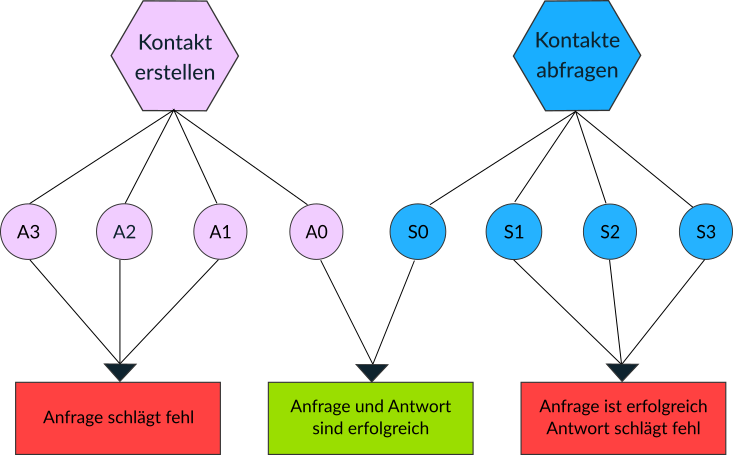
\includegraphics[width=0.8\textwidth]{Szenarien}
  \grayRule
  \caption[Szenarien]{Szenarien und Fälle}
  \label{fig:scenarios}
\end{figure}
%
% ERGEBNIS
%
\subsection*{Ergebnis}
Da die Szenarien \it{A0} und \it{S0}, die Szenarien \it{A1}, \it{A2} und \it{A3} sowie die Szenazien\it{S1}, \it{S2} und \it{S3} zusammengefasst werden können, ergeben sich aus den acht Szenarien die drei nun aufgezählten Fälle.
\begin{itemize}
  \item Fall a: Anfrage und Antwort sind erfolgreich. Es besteht kein Aktionsbedarf \highlight{irrelevant?}
  \item Fall b: Anfrage ist nicht erfolgreich
  \item Fall c: Anfrage ist erfolgreich, Antwort schlägt fehl
\end{itemize}
\highlight{Ergebnis für Fall b und c ist nur aus Entwicklungsperspektive (für die Behandlung) interessant. Das Ergebnis ist identisch: fail}\\
\todo{Anforderungen:}
\it{Die Daten sollten wenigstens so lange auf dem Client gespeichert werden, bis sie vollständig beim Server angekommen sind. Jeder Fehlersfall muss kommuniziert werden. Wenn es konliktbehaftete Daten gibt muss dies mitgeteilt, und angeboten werden die Konflikte zu lösen (Welche Telefonnummer ist die richtige).}\\
Im weiteren Verlauf dieser Arbeit wird unter anderem beschrieben, wie diese Fälle \ldots  eingebunden werden.
\chapter{\label{chap:anforderungen}Anforderungsdefinition}
Dieses Kapitel beschreibt die Anforderungen an eine Offline First Anwendung unter Berücksichtigung von Konfliktmanegement und Funktionalität.
Die von BenutzerInnen generierten Daten sollten wenigstens so lange auf dem Client gespeichert werden, bis sie vollständig beim Server angekommen sind. Jeder Fehlersfall muss kommuniziert werden. Wenn es konliktbehaftete Daten gibt muss dies mitgeteilt, und angeboten werden die Konflikte zu lösen (Welche Telefonnummer ist die richtige).\\
Aus den oben genannten \hyperref[chap:szenarien]{Szenarien} werden im Folgenden die Anforderungen hergeleitet, die eine offlinefähige Anwendung \highlight{unter Berücksichtigung von...} erfüllen soll.
\begin{enumerate}
  \item Nur die Einträge laden die ich noch nicht hab
    \subitem kostet Bandbreite und Serverarbeitszeit
    \subitem doppelt (geladen)
    \subitem dauert länger (response)
  \item Einträge identifizieren (key)
    \subitem Operationen müssen dem Objekt/Eintrag zugeordnet werden
  \item Delta berechnen
  \item lokal und auf dem Server gespeichert sein
  \item 2 Objekte mit derselben ID ? welches ist das aktuellste
  \item mehr als 2 Objekte mit derselben ID ? sortieren
  \item Liste von inhaltsbasierten Versionen muss festgelegte Länge haben
  \item Konflikte effizient speichern
  \item
\end{enumerate}
\todo{Damit ein Datensatz, wie zum Beispiel ein Adressbucheintrag, offline erreichbar sind, muss er sowohl auf dem Client, als auch auf dem Server gespeichert sein. Im aktuellen Anwendungsfall bedeutet das, es gibt zwei Kopien des Adressbucheintrags. Eine auf dem Anwendungsgerät, eine auf dem Server.\\
Um dieses Delta zu kalkulieren müssen Daten auf dem Client gespeichert werden (localStorage, lokale Datenbank oder Datei...) | Server muss die Daten sortieren können und in der Lage sein nur bestimmte Daten zu liefern.}
%
% Use Cases  \hyperref[sec:conflict]{oben}
%
\section{Anwendungsfälle}
Aus den in Kapitel \ref{chap:szenarien} erarbeiteten Szenarien ergeben sich die folgenden Use-Cases, die von einer offlinefähigen Anwendung erfüllt werden sollen. Die folgende Tabelle zeigt die Anwendungsfälle aus der Entwicklungsperspektive.
\begin{longtable}[c]{@{}
>{\columncolor[HTML]{CFFCC2}}l ll@{}}
\toprule
    \multicolumn{1}{p{0.1\textwidth}}{\cellcolor[HTML]{cffcc2}\textbf{ID}}
    & \multicolumn{1}{p{0.45\textwidth}}{\cellcolor[HTML]{cffcc2}\textbf{Anwendungsfall}}
    & \multicolumn{1}{p{0.45\textwidth}}{\cellcolor[HTML]{cffcc2}\textbf{Beschreibung}}\\ \hline
\endfirsthead
%
\endhead
%
  \multicolumn{1}{l}{\cellcolor[HTML]{cffcc2}\textbf{UC1}} &
  \multicolumn{1}{p{0.45\textwidth}}
  {Um die Anwendung auch ohne Internetzugang zu nutzen, sollen die Daten auch offline erreichbar sein.}
  & \multicolumn{1}{p{0.45\textwidth}}
  {Die Daten werden auf dem Server und lokal gespeichert. Lokal bedeutet in einer lokalen Datenbank oder im Browser (localStorage, IndexedDB usw.).}\\
  \midrule
  %
  \multicolumn{1}{l}{\cellcolor[HTML]{cffcc2}\textbf{UC2}} &
  \multicolumn{1}{p{0.45\textwidth}}
  {Die Anwendung soll die Kontaktliste schnell und effizient laden.}
  % {Um Datentraffic und Ladezeiten zu sparen / schnell und effizient möchte ich nur die Adressbucheinträge oder deren Aktualisierungen laden, die sich nicht schon auf dem Endgerät befinden.}
  & \multicolumn{1}{p{0.45\textwidth}}
  % {Es wird ermittelt welche Daten neu angelegt oder aktualisiert wurden. Dazu müssen sie sortierbar und versionierbar sein.}\\
  {Es werden nur Einträge oder deren Aktualisierungen geladen, die sich noch nicht auf dem Endgerät befinden.}\\
  \midrule
  %
  \multicolumn{1}{l}{\cellcolor[HTML]{cffcc2}\textbf{UC3}} &
  \multicolumn{1}{p{0.45\textwidth}}
  {Ich möchte Einträge immer und überall editieren können.}
  & \multicolumn{1}{p{0.45\textwidth}}
  {Jeder Eintrag muss identifizierbar und versionierbar sein.}\\
  \midrule
  %
  \multicolumn{1}{l}{\cellcolor[HTML]{cffcc2}\textbf{UC4}} &
  \multicolumn{1}{p{0.45\textwidth}}
  {Um jedem Adressbucheintrag Operationen zuzuweisen und einzelne Kontakte zu finden, möchte ich die Einträge identifizieren.}
  & \multicolumn{1}{p{0.45\textwidth}}
  {Jeder Eintrag bekommt zur eindeutigen Identifikation eine \gls{UUID} zugewiesen.}\\
  \midrule
  %
  \multicolumn{1}{l}{\cellcolor[HTML]{cffcc2}\textbf{UC5}} &
  \multicolumn{1}{p{0.45\textwidth}}
  {Um zu wissen ob, wie oft und wann ein Eintrag bearbeitet wurde, möchte ich die Einträge versionieren.}
  & \multicolumn{1}{p{0.45\textwidth}}
  {Jeder Eintrag bekommt ein Versionsattribut.}\\
  \midrule
  % UC6
  \multicolumn{1}{l}{\cellcolor[HTML]{cffcc2}\textbf{UC6}} &
  \multicolumn{1}{p{0.45\textwidth}}
  {Ich möchte dass alle Änderungen ankommen und keine Daten verloren gehen.}
  &
  \multicolumn{1}{p{0.45\textwidth}}
  {Wenn ein Konflikt auftritt, wird er effizient gespeichert (statt eine Version zu verwerfen).}\\
  \midrule
  % UC7
  \multicolumn{1}{l}{\cellcolor[HTML]{cffcc2}\textbf{UC7}} &
  \multicolumn{1}{p{0.45\textwidth}}
  {Ich weiß, Konflikte können immer auftreten, deswegen möchte ich mit ihnen umgehen können.}
  & \multicolumn{1}{p{0.45\textwidth}}
  {Konflikte werden effizient gespeichert, sodass sie nach und nach von NutzerInnen aufgelöst werden können.}\\
  % end
  \bottomrule \cellcolor[HTML]{FFFFFF}
  \vspace{0.1cm}\\
  \noalign{\hspace{0.0525\textwidth}\grayRule}
  \caption{Anwendungsfälle}
  \label{tab:uc}\\
\end{longtable}

Das in Abbildung \ref{fig:uc} gezeigte Use-Case-Diagramm veranschaulicht die in der obigen Tabelle \ref{tab:uc} aufgeführten Anwendungsfälle.
\begin{figure}[H]
    \centering
    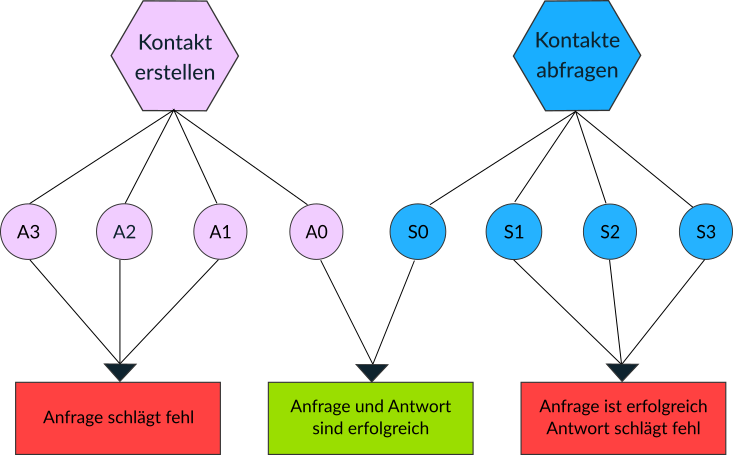
\includegraphics[width=\textwidth]{Szenarien}
    \grayRule
    \caption[Use-Case Diagramm]{Platzhalter für UC-Diagramm}
    \label{fig:uc}
\end{figure}
%
% Funktionalität
%
\section{Funktionalität}
\todo{siehe Anforderungen PWA?} Plus kein Datenverlust, und 'just work'\\
Daten sollen, sobald einmal geladen, auch offline verfügbar sein.
Daten sollen jederzeit (offline und online) lesbar und bearbeitbar (löschbar) sein.
%
% UI
%
\section{Die graphische Oberfläche}
\Gls{optimistic UI}
\gls{UI} soll mich nicht mit Meldungen darüber nerven, dass ich offline bin. (Bsp. Chat)\\
\gls{UI} soll sagen wenn es einen Konflikt gab / gibt und mich entscheiden lassen. Bzw ihn lösen lassen.
Auf keinen Fall selber lösen und mich nichts davon wissen lassen.\\
Im besten Fall soll due UI mir sagen \b{warum} es zum Konflikt gekommen ist.
\chapter{\label{chap:konzeption}Konzeption}
Die erarbeiteten Anforderungen an [...] werden in diesem Kapitel für die Konzeption angewendet. Beginnend mit dem Aufbau der Anwendung werden in den folgenden Abschnitten das Design, die von der Anwendung genutzten Daten, Anwendungsfälle, die Architektur und schließlich die Komponenten der Entwicklumgsumgebung aufgeführt.
\section{Anwendungsaufbau}
\section{Datengrundlage}

\section{Anwendungsfälle}
Aus den in Kapitel \ref{chap:anforderungen} beschriebenen Anforderungen und den in Kapitel \ref{chap:szenarien} erarbeiteten Szenarien ergeben sich die folgenden [zahl] Use-Cases, die von der Anwendung erfüllt werden sollen.\\

\section{Architektur}
%\clearpage
\section{Die graphische Oberfläche}

% TESTFÄLLE
\section{Testfälle}
olgende Testfälle werden während der Entwicklung stetig durchgeführt. Das erfolgreiche Bestehen dieser Tests ist eine notwendige Qualitätseigenschaft der zu entwickelnden Applikation.


%
% Entwicklungsumgebung
%
\clearpage
\section{Entwicklungsumgebung}
Für die Erstellung der Smartphone-Applikation wurde folgende Soft- und Hardware verwendet:
\subsubsection{Software}
\begin{itemize}
	\item Android Studio\footnote{ Download unter \url{http://developer.android.com/sdk/index.html}} Version 1.1. Enthält Android Studio IDE, Android \gls{SDK}-Tools, Android 5.0 Plattform, Android 5.0 Emulator System Image mit Google \glspl{API}
	\item Sublime Editor 3
	\item git, Version 1.7.10.4 zur Versionsverwaltung
	\item Google Drive zur Erstellung der Diagramme, Zeichnungen und Grafiken
\end{itemize}
\subsubsection{Hardware}
\begin{itemize}
	\item Tuxedo  (Intel\textsuperscript{\textregistered} Core\texttrademark   i7-6500U, 2,50GHz x 4, 7,7 GB RAM) als ersten Entwicklungsrechner (Betriebssystem: Ubuntu\footnote{ Download unter \url{https://www.ubuntu.com/download/desktop}} 16.06, 64-bit-Version)
	\item Lenovo Thinkpad X200 (Intel\textsuperscript{\textregistered} Core\texttrademark   2 Duo, 2,40GHz, 8GB RAM) als zweiten Entwicklungsrechner (Betriebssystem: Debian 7.8, 64-bit-Version)
	\item Android Testgeräte: Samsung Galaxy Note 2, Samsung Nexus S, LG Nexus 4, LG Nexus 5, HTC Desire HD
\end{itemize}

\chapter{\label{chap:implementierung}Implementierung}
\section{Installation}
\sub{1}
\subsub{Pouch}
\subsub{Couch}
\sub{2}
%
% Installationsanleitung
%
\section{Installationsanleitung}
Beide entwickelten Prototypen sind als öffentliche Repositories auf GitHub\footnote{Software--Entwicklungs--Plattform \url{https://github.com/}} zu finden. 
Um sie zu installieren müssen folgende Schritte ausgeführt werden.
\sub{amilia-qouch}
1. Zuerst muss das Repository kopiert werden:
\lstset{language=sh, caption={},belowcaptionskip=0.3\baselineskip}
\begin{lstlisting}
git clone git@github.com:hulkoba/amilia-qouch.git
# oder
git clone https://github.com/hulkoba/amilia-qouch.git
\end{lstlisting}
2. Dann muss man in das Verzeichnis navigieren und alle Abhängigkeiten installieren.
\begin{lstlisting}
cd amilia-qouch
npm install
\end{lstlisting}
3. Mittels
\begin{lstlisting}
npm start
\end{lstlisting}
wird die Anwendung gestartet.
%
\sub{amilia-rdx}
1. Auch hier muss das Repository zuerst kopiert werden:
\lstset{language=sh, caption={},belowcaptionskip=0.3\baselineskip}
\begin{lstlisting}
git clone git@github.com:hulkoba/amilia-rdx.git
# oder
git clone https://github.com/hulkoba/amilia-rdx.git
\end{lstlisting}
2. Schritt zwei ist identisch mit dem in der \tt{amilia-qouch} Anleitung\\
3. Mittels
\begin{lstlisting}
npm run server
npm start
\end{lstlisting}
wird zuerst der Server, dann die Anwendung gestartet.
\chapter{\label{chap:evaluation}Evaluation}
Um die Funktionalität des Prototyps zu untersuchen, wurden folgende Testgeräte ausgewählt.
%
% Systemtest
%
\section{Systemtest und Ergebnisse}

\section{Vergleich}
\begin{longtable}[c]{@{}
	>{\columncolor[HTML]{CFFCC2}}l ll@{}}
	\toprule
	\multicolumn{1}{p{0.1\textwidth}}{\cellcolor[HTML]{cffcc2}{}} 
  &
	\multicolumn{1}{p{0.45\textwidth}}{\cellcolor[HTML]{cffcc2}\textbf{PouchDB}}
	&
  \multicolumn{1}{p{0.45\textwidth}}{\cellcolor[HTML]{cffcc2}\textbf{Redux Offline}} \\
	
  \hline \noalign{\vskip 0.1cm}
	\endfirsthead
	\endhead
	%
\multicolumn{1}{p{0.1\textwidth}}
{\textbf{Storage}}
&       
\multicolumn{1}{p{0.45\textwidth}}
{IndexedDB WebSQL}
&                                                                                         
\multicolumn{1}{p{0.45\textwidth}}
{(redux-persist) Brwoser: IndexedDB oder WebSQL / LocalStorage, Fallbacks via localForage.
ReactNative: AsyncStorage}\\
\midrule
% ----------------------------------------------
\multicolumn{1}{p{0.1\textwidth}}
{\textbf{Requirements}}
&       
\multicolumn{1}{p{0.45\textwidth}}
{--}
&                                                                                         
\multicolumn{1}{p{0.45\textwidth}}
{Redux}\\
\midrule
% ----------------------------------------------
\multicolumn{1}{p{0.1\textwidth}}
{\textbf{Lines of Code}}
&       
\multicolumn{1}{p{0.45\textwidth}}
{?}
&                                                                                         
\multicolumn{1}{p{0.45\textwidth}}
{?}\\
\midrule

	%
	% end
	\bottomrule \cellcolor[HTML]{FFFFFF}
	\vspace{0.1cm}\\
	\noalign{\hspace{0.0525\textwidth}\grayRule}
	\caption{Anforderungen aus Entwicklungsperspektive}
	\label{tab:evaluation}\\
\end{longtable}

\chapter{\label{chap:fazit}Zusammenfassung und Ausblick}
Interessant wäre es andere Datenbanklösungen zu untersuchen.
Realm ist leider kostenpflichtig, wäre aber äußerst spannend weil Realm so viel verspricht.

%
%	APPENDICES
%

%% Ein kleiner Abstand zu den Kapiteln im Inhaltsverzeichnis (toc)
\addtocontents{toc}{\protect\vspace*{\baselineskip}}


\printglossary[type=\acronymtype, title=Abkürzungen, style=super]
\printglossary[type=main,style=altlist]

%
%Abbildungsverzeichnis
%
\clearpage
\addcontentsline{toc}{chapter}{Abbildungsverzeichnis}
\listoffigures

% \renewcommand\lstlistlistingname{Quellcodeverzeichnis} %Inhaltsverzeichnistitel = Inhalt
%\lstlistoflistings%quellcodeverzeichnis

% Literaturverzeichnis
\addcontentsline{toc}{chapter}{Literaturverzeichnis}
\bibliographystyle{alphadin}
\bibliography{appendices/literatur}


% Anhang
\clearpage
\appendix
\addcontentsline{toc}{chapter}{Anhang}
\chapter*{Anhang}
\section*{Eidesstattliche Erklärung}
\section*{CD-Inhalt}
Auf der beigefügten CD befinden sich
\begin{itemize}
	\item Die schriftliche Ausarbeitung dieser Bachelorarbeit im PDF-Format
	\item Das erstellte Projekt	inklusive der Android .apk-Datei
	\item Testprotokolle
\end{itemize}


\end{document}
